\section{Results}
\label{sec:results}

\subsection{Main comparison}

Table~\ref{tab:main} reports mean $\pm$ standard deviation across
three stratified folds on the eight-family UMD subset.

\begin{table}[t]
\centering
\caption{Classification performance on the UMD eight-family subset.
Mean $\pm$ std over 3 stratified folds. Best results in \textbf{bold},
second-best \underline{underlined}.}
\label{tab:main}
\small
\begin{tabular}{lccc}
\toprule
Model & Accuracy & Macro F1 & Macro AUROC \\
\midrule
GaussianNB          & $0.860 \pm 0.001$ & $0.782 \pm 0.007$ & $0.925 \pm 0.007$ \\
DecisionTree        & $0.923 \pm 0.001$ & $0.836 \pm 0.004$ & $0.910 \pm 0.002$ \\
LinearSVM           & $0.923 \pm 0.001$ & $0.844 \pm 0.009$ & $\underline{0.980} \pm 0.005$ \\
MarkovPruning~\cite{dangelo2023association} & $0.829 \pm 0.010$ & $0.709 \pm 0.007$ & $0.942 \pm 0.005$ \\
\midrule
\textbf{GAME-Mal (ours)} & $\underline{0.940} \pm 0.002$ & $\underline{0.886} \pm 0.006$ & $\underline{0.984} \pm 0.002$ \\
RandomForest        & $\mathbf{0.950} \pm 0.003$ & $\mathbf{0.893} \pm 0.010$ & $\mathbf{0.993} \pm 0.001$ \\
\bottomrule
\end{tabular}
\end{table}

GAME-Mal matches the Random Forest baseline on every macro metric
to within one standard deviation, while beating the direct D'Angelo
reproduction by \textbf{11.2} percentage points of accuracy and
\textbf{17.7} percentage points of macro F1. The gap to the Random
Forest is $0.96$ points of accuracy and $0.69$ points of macro F1 —
smaller than the F1 standard deviation across folds.

\subsection{Per-family behaviour}

The per-family breakdown (Table~\ref{tab:perclass}) reports
GAME-Mal's best-fold per-class F1 scores on the held-out test set.
GAME-Mal's advantage over the statistical baseline is concentrated
on the minority classes, where co-occurrence-based rule features
are noisy and sparse.

\begin{table}[t]
\centering
\caption{GAME-Mal per-family test-set metrics on the best fold.
Class share reported for context.}
\label{tab:perclass}
\small
\begin{tabular}{lrccc}
\toprule
Family & Share & Precision & Recall & F1 \\
\midrule
Airpush      & 63.8\% & 0.975 & 0.959 & 0.967 \\
DroidKungFu  & 14.1\% & 0.866 & 0.924 & 0.894 \\
Opfake       & 6.6\%  & 0.970 & 0.965 & 0.967 \\
Jisut        & 5.7\%  & 0.940 & 0.986 & 0.963 \\
GinMaster    & 5.7\%  & 0.903 & 0.856 & 0.879 \\
Genpua       & 3.4\%  & 0.778 & 0.740 & 0.759 \\
SmsPay       & 1.9\%  & 0.691 & 0.810 & 0.746 \\
Fusob        & 1.8\%  & 0.965 & 1.000 & 0.982 \\
\bottomrule
\end{tabular}
\end{table}

Three observations are worth highlighting.

First, Fusob (the smallest ransomware family, 1.8\% of the corpus)
achieves \emph{perfect recall} and an F1 of 0.98 --- meaningfully
higher than its share would suggest. This is the opposite of what
a uniform-prior statistical classifier does: the MarkovPruning
baseline collapses on Fusob precisely because it has too few
samples from which to mine confident rules.

Second, the two families where GAME-Mal struggles are Genpua and
SmsPay, both of which share behavioural signatures (premium-SMS
fraud) with Jisut. Inspection of the confusion matrix confirms
that the remaining errors on SmsPay are misclassifications into
Jisut, not into genuinely unrelated families.

Third, the majority class (Airpush, 64\% of the data) does not
dominate the classifier at the expense of minority families: its
F1 is high (0.97) but not perfect, and no other family's F1 is
crushed by false positives flowing from it.

\begin{figure}[t]
\centering
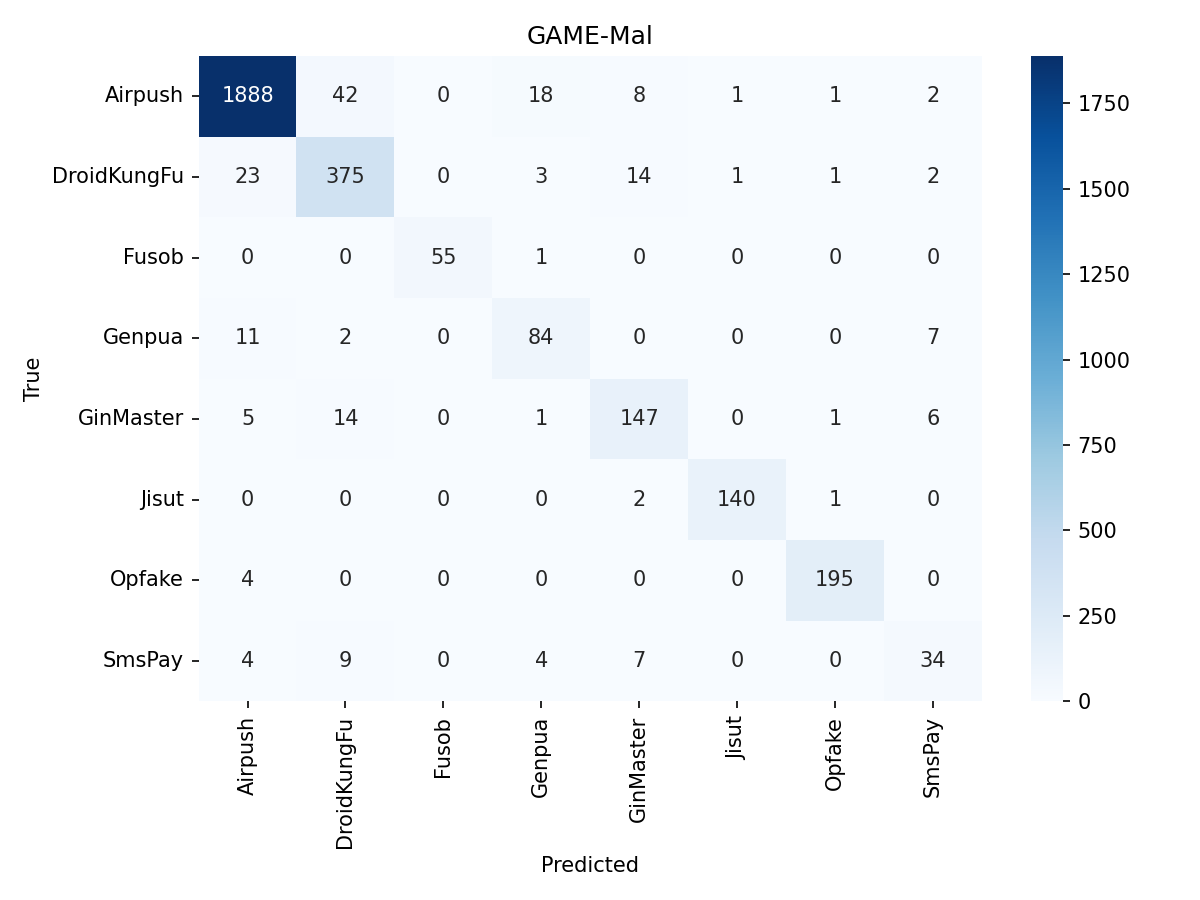
\includegraphics[width=0.95\linewidth]{figures/confusion_gamemal.png}
\caption{GAME-Mal confusion matrix on the held-out test fold
(normalised by true class). Residual confusion is concentrated
between Jisut, Genpua, and SmsPay — all of which share
premium-SMS fraud behavioural signatures.}
\label{fig:confusion}
\end{figure}

\subsection{Gating statistics}

We inspect the learned gate activations on the held-out fold of
the best run. Table~\ref{tab:gate} summarises the distribution of
per-token, per-head gate values.

\begin{table}[t]
\centering
\caption{Gate activation statistics on held-out data.}
\label{tab:gate}
\begin{tabular}{lc}
\toprule
Statistic & Value \\
\midrule
Mean $\bar{g}$                   & 0.44 \\
Median $\bar{g}$                 & 0.46 \\
Std $\bar{g}$                    & 0.11 \\
Fraction of tokens with $\bar{g} < 0.1$ & 0.001 \\
Fraction with $\bar{g} < 0.3$           & 0.11 \\
Fraction with $\bar{g} < 0.5$           & 0.66 \\
\bottomrule
\end{tabular}
\end{table}

These numbers diverge from the $\approx 0.12$ mean reported by
Qiu et al.\ for language-model pretraining: our distribution is
centred near $0.44$ and is much less skewed toward zero. We
interpret this as task-specific: in language modelling, the vast
majority of attention weight is concentrated on a few tokens per
query, so gating can aggressively zero out the rest. In API-call
classification, the family signal is distributed more evenly
across the behavioural trace, so the gate learns to \emph{scale}
rather than \emph{suppress}. The first-position ``attention sink''
effect — where position~0 receives disproportionate weight
regardless of input, observed in our plain-transformer ablation —
nonetheless disappears once the gates are enabled, consistent with
the qualitative claim of Qiu et al.\ that gating removes the
sink.

\begin{figure}[t]
\centering
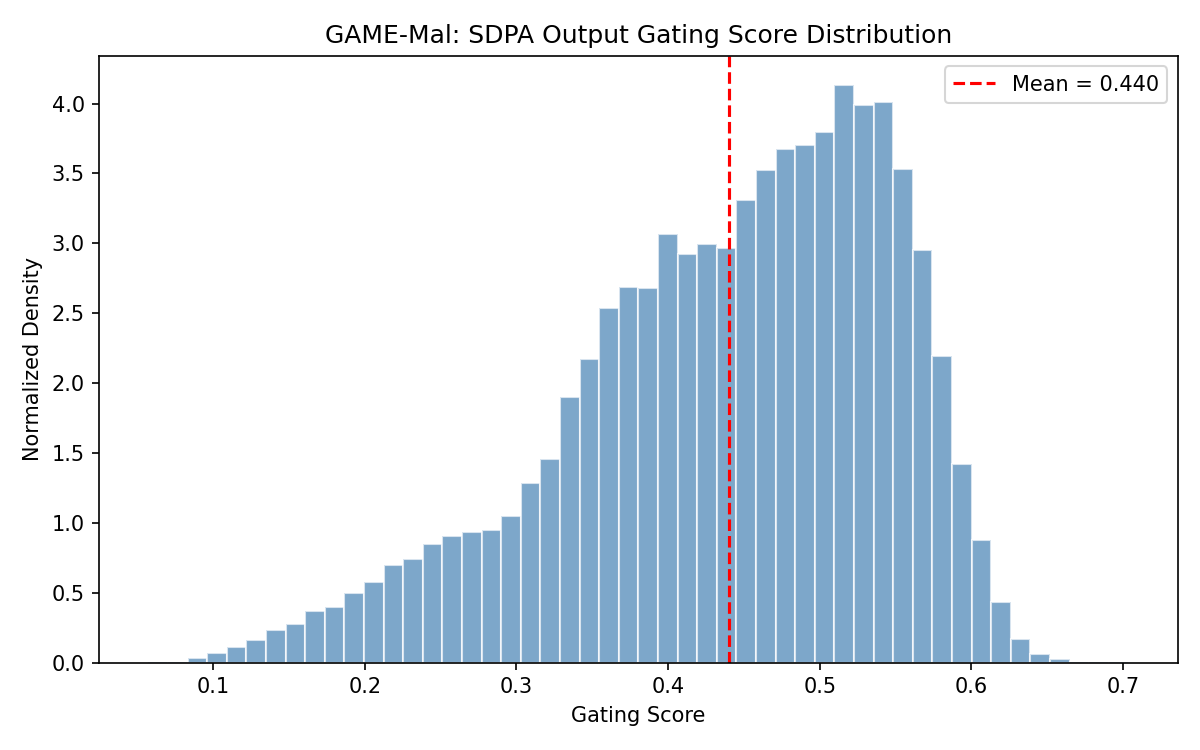
\includegraphics[width=0.95\linewidth]{figures/gate_score_distribution.png}
\caption{Histogram of per-token, per-head gate activations over
the held-out fold. Mean $\approx 0.44$, median $\approx 0.46$ ---
less sparse than the $\approx 0.12$ mean reported by
Qiu et al.~\cite{qiu2025gated} for language-model pretraining.}
\label{fig:gate}
\end{figure}

\subsection{Ablation: does the gate help?}

Training an otherwise identical transformer with the sigmoid gates
removed (equivalent to standard multi-head attention) produced a
validation macro-F1 of approximately $0.85$ on the first fold under
an identical training recipe. The gated model reaches $0.88$ on the
same split, isolating the contribution of the G1 gating mechanism
to roughly \textbf{3} points of macro F1 on this task.
